% Section: who gains and who loses (input by mfg/paper/main.tex); numbers from mfg/paper/numbers_stake.tex
\section{Who gains and who loses}\label{sec:stake}

The welfare results above add up three groups: carriers, buyers of deliveries and the city. This section separates them. The accounting is that of Section~\ref{sec:model}: in zone-hour $k$ the price is $\alpha_k-b_kQ_k$, a delivery carries the delay cost $\kappa_kQ_k$, and the city posts a charge $u_k$ per delivery. For a profile with aggregate $Q$ and carrier profit vector $\pi$,
\begin{align*}
\text{consumer surplus } \mathrm{CS}&=\tfrac12\ip{b}{Q^2}, & \text{congestion cost } \mathrm{CC}&=\ip{\kappa}{Q^2},\\
\text{charge revenue } R&=\ip{u}{Q}, & \text{carrier profit } \Pi&=\sum_i\pi_i-\ip{b}{Q^2}-\mathrm{CC}-R,
\end{align*}
and $\SW=\mathrm{CS}+\Pi+R$ exactly (unit test in \texttt{mfg/tests/test_stake.py}; the identity holds to \StakeIdErr{} relative error in all \StakeRows{} instances). Charges are a transfer: they move welfare between $\Pi$ and $R$ and change $\SW$ only through the deliveries. In this model the delay cost is borne by the delivery fleet, so residents carry no monetary congestion cost; their stake is the demand side (CS) and, in Section~\ref{sec:residents}, the vehicle-hours spent in their zone.

\paragraph{Three rules} All rules are evaluated at the Nash equilibrium of the finite market under the posted charge, on the instances of Section~\ref{sec:exp} (nine cities, five seeds, $N=6k$, $k=1,\dots,256$). \emph{No charge}: $u=0$. \emph{Observation-only}: the finite-market fixed point $u=\kappa\odot Q(u)$ of Proposition~\ref{prop:arp}, the Pigou charge without any market-power correction. \emph{Pigou minus market power} (the rule of the Omega paper): $u=\kappa\odot Q^\opt-m\odot\bar a$, with $\bar a_k$ the optimum's delivery per active carrier, corrected for 25 damped rounds $u\leftarrow u+0.8\,m\odot(1+1/n_k)\odot(Q(u)-Q^\opt)$ ($n_k$ the number of active carriers) so that the Nash aggregate matches $Q^\opt$; the median relative $M$-norm residual of the match is \PmResidMed{} (maximum \PmResidMax). This rule solves for a charge that reproduces the optimal aggregate; with several carrier types it need not reproduce the optimal individual plans, so it can fall short of $\SW^\opt$ (median welfare shortfall \PmLossSix\% at $N=6$ and \PmLossBig\% at $N=1536$).

\subsection{The charge that implements the optimum}\label{sec:ident}
For one segment split into $N$ identical carriers the optimal charge has a closed form.

\begin{proposition}[Pigou minus market power]\label{prop:marketpower}
Let the $N$ carriers be identical replicas of one type (Lemma~\ref{lem:rep}) and let $Q^\opt$ be the aggregate of a social optimum. The charge
\[
u^*_N=\kappa\odot Q^\opt-\tfrac1N\,m\odot Q^\opt
\]
makes the Nash equilibrium aggregate equal to $Q^\opt$ and its welfare equal to $\SW^\opt$, for any coupling of the plans across zone-hours. It is the Pigou charge $\kappa\odot Q^\opt$ minus a market-power term of exact size $\tfrac1N m_kQ^\opt_k$. Coordinate $k$ is taxed if $N>m_k/\kappa_k=1/\varrho_k$ and subsidised if $N<1/\varrho_k$. In the one-zone case with unconstrained deliveries, $Q^\Nash=\frac N{N+1}Q^\War$, $Q^\War=\alpha/m$, $Q^\opt=\alpha/(m+\kappa)$ and $u_N^*=\alpha(\kappa-m/N)/(m+\kappa)$.
\end{proposition}
\begin{proof}
By Lemma~\ref{lem:rep} with one type, the type total $Y$ of a Nash equilibrium maximises $\Phi(Y)=\pi(Y)-\ip{u}{A}-\tfrac12(1+\tfrac1N)\norm{A}_m^2$, $A=LY$, over the (convex) fleet polytope, and each carrier delivers $A/N$. At $u=u_N^*$ the gradient of $\Phi$ at the social optimum $Y^\opt$ is $\nabla\pi-L^\top[(\kappa-\tfrac mN)\odot Q^\opt+(1+\tfrac1N)m\odot Q^\opt]=\nabla\pi-L^\top[(m+\kappa)\odot Q^\opt]$, which is the gradient of the social objective $\pi-\tfrac12\norm{A}_{m+\kappa}^2$ at $Y^\opt$. The variational inequality of $Y^\opt$ for the social problem is therefore that of $\Phi$; $\Phi$ is concave, so $Y^\opt$ maximises it, and the Nash aggregate is unique (Lemma~\ref{lem:pot}(b)). Welfare depends on the profile only through $\pi$ and $Q$. The one-zone formulas: the Nash first-order condition $\alpha-u=(1+\tfrac1N)mQ$ gives $Q^\Nash=\frac N{N+1}\alpha/m$ at $u=0$, and $u=\alpha-(1+\tfrac1N)m\frac{\alpha}{m+\kappa}=\alpha\frac{\kappa-m/N}{m+\kappa}$ at $Q=Q^\opt$.
\end{proof}

The proposition was checked on the nine cities with one segment per city (three seeds, $N=1,2,3,6,\dots,1536$, \IdRows{} instances): the Nash aggregate under $u_N^*$ equals $Q^\opt$ to a relative $M$-norm error of at most \IdQErr{} and the welfare to \IdSWErr{}, while without a charge a single-segment market loses \IdSixNone\% of optimal welfare at $N=6$ (median) and the pure Pigou charge \IdSixPig\%; at $N=1536$ the losses are \IdBigNone\% and $4\cdot10^{-5}\%$. The charge is a subsidy in every zone-hour at $N=6$ and in \IdOneNinetyTwoSub\% of them at $N=192$; its size relative to the Pigou charge is \IdSixRatio{} at $N=6$ (the sum over zone-hours, a net subsidy) and \IdBigRatio{} at $N=1536$. The one-zone relation $Q^\Nash=\frac N{N+1}Q^\War$ is exact only while the fleet budget is slack: it holds to $10^{-9}$ in six of the nine cities and deviates by up to \IdRatioDevMax\% elsewhere, where the budget binds; the charge formula does not depend on it. For several carrier types the charge $u^*_N$ is not available, because the market-power terms $m\odot a_\theta$ differ across types and one posted charge cannot cancel all of them; the rule above is the numerical substitute.

\subsection{The city council}\label{sec:council}
Table~\ref{tab:stake_who} gives, for the four sizes $N\in\{6,24,192,1536\}$ and the two rules that charge, the change of each term relative to no charge, as a percentage of welfare without charge (medians over nine cities and five seeds; city values in \texttt{results/summary\_stake\_who\_city.csv}). Figure~\ref{fig:stake_who} shows all nine sizes.

\begin{table}[t]
\centering\footnotesize\setlength{\tabcolsep}{4pt}
\caption{Change with respect to no charge, in \% of welfare without charge (median of 45 instances). $\Delta\Pi$: carrier profit net of the charge; $\Delta$CS: consumer surplus; $\Delta$CC: congestion cost; $R$: charge revenue (negative: subsidy paid by the city); $\Delta\SW=\Delta\Pi+\Delta\mathrm{CS}+R$ up to medians; last column: $R$ as a share of the welfare under the rule.}\label{tab:stake_who}
\begin{tabular}{rlrrrrrr}
\toprule
$N$ & rule & $\Delta\Pi$ & $\Delta$CS & $\Delta$CC & $R$ & $\Delta\SW$ & $R/\SW$\\
\midrule
6 & observation-only & -1.1 & -1.0 & 0.0 & +1.6 & -0.5 & +1.6 \\
 & Pigou minus market power & +132.0 & +69.1 & +2.2 & -181.9 & +19.6 & -151.9 \\
\addlinespace
24 & observation-only & -0.7 & -2.4 & -0.1 & +2.7 & -0.3 & +2.8 \\
 & Pigou minus market power & +13.4 & +21.6 & +0.7 & -36.9 & +1.9 & -36.1 \\
\addlinespace
192 & observation-only & -0.4 & -1.8 & -0.1 & +3.3 & 0.0 & +3.3 \\
 & Pigou minus market power & +0.3 & +0.1 & 0.0 & -1.9 & 0.0 & -1.9 \\
\addlinespace
1536 & observation-only & -0.1 & -1.6 & -0.1 & +3.4 & 0.0 & +3.4 \\
 & Pigou minus market power & -0.1 & -1.1 & -0.1 & +3.0 & 0.0 & +3.0

\bottomrule
\end{tabular}
\end{table}

\begin{figure}[t]
\centering
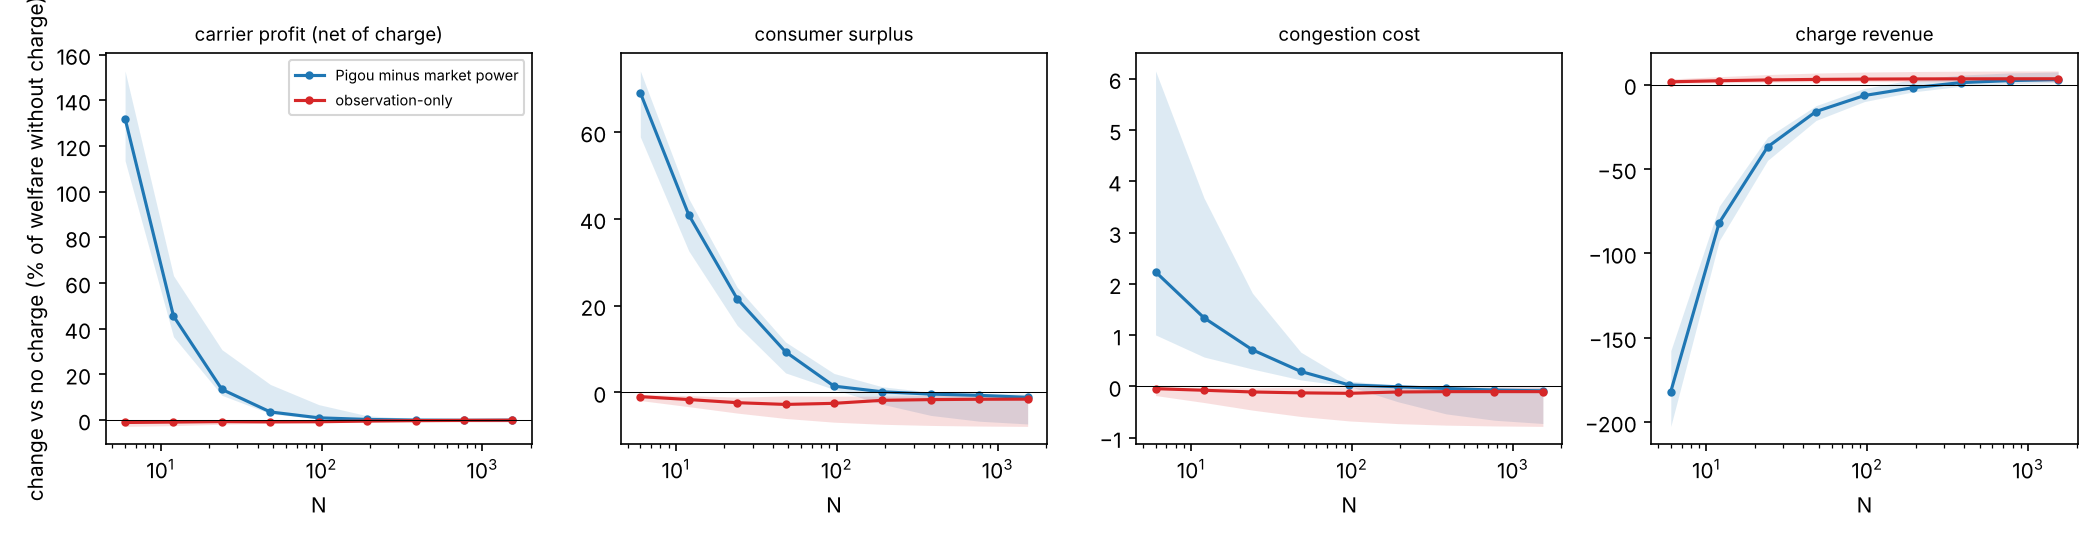
\includegraphics[width=\textwidth]{mfg_stake_who.png}
\caption{Change of each welfare term against no charge (\% of welfare without charge; median and interquartile range over nine cities and five seeds). Blue: Pigou minus market power; red: observation-only.}\label{fig:stake_who}
\end{figure}

\paragraph{Revenue} With many carriers the council collects about \WBigObsR\% of welfare under either rule (the Pigou charge in the limit), \WBigPmRshare\% under the market-power rule at $N=1536$. With few carriers the picture reverses. The observation-only charge still raises \WSixObsR\% of welfare but lowers welfare by \WSixObsdSW\% (it taxes deliveries that Cournot carriers already withhold), whereas the market-power rule raises welfare by \WSixPmdSW\% at a net \emph{cost} to the council: its revenue is $\WSixPmR\%$ of the no-charge welfare, i.e.\ \WSixPmRshare\% of the welfare under the rule, and it is negative in \PmSubsidyInst{} instances. The efficient charge at $N=6$ is a subsidy to carriers in about \PmNegShare\% of zone-hours; it removes the market power by paying carriers to deliver more. At $N=24$ the subsidy is still $36.9\%$ of the no-charge welfare and it falls under $2\%$ at $N=192$. A council that cannot run a deficit has to recover the transfer by a lump-sum fee (a fixed licence fee does not change the deliveries; not modelled here), or settle for a smaller correction. Budget neutrality is thus a property of large markets only.

\paragraph{One city-wide charge or zone-hour charges?} The market-power charge is posted per zone and hour. If the council may post a single per-delivery charge $\bar u$ for the whole city, the best scalar (found by a grid and a bounded search; \texttt{results/uniform.csv}) leaves a welfare loss of \UnSixUni\% of the optimum at $N=6$ against \UnSixPm\% for zone-hour charges and \UnSixNone\% without charge; it captures \UnSixFrac\% of the gain of the zone-hour rule (median; range \UnSixFracMin--\UnSixFracMax\%). The best scalar is negative, a subsidy, for small $N$ and turns positive near $N=16$ to $32$. In the mean-field limit the loss of the best single charge is \UnWUni\% of the optimum (maximum \UnWUniMax\%) against $0$ for zone-hour charges, and no charge loses \UnWNone\%: the best city-wide charge captures \UnWFrac\% of the possible gain (range \UnWFracMin--\UnWFracMax\%). Differentiated charges therefore matter most where the calibrated congestion slopes differ most across zone-hours; with this calibration the welfare at stake in the choice is small in absolute terms.

\paragraph{A wrong charge} Let the council post $(1+\varepsilon)$ times the Pigou charge, $\varepsilon\in\{\pm10\%,\pm25\%\}$, in the mean-field market. Theorem~\ref{thm:welfare}(a) bounds the loss by $\tfrac12\norm{v-\kappa\odot Q^\opt}_{b^{-1}}^2=\tfrac12\varepsilon^2\norm{\kappa\odot Q^\opt}^2_{b^{-1}}$. Measured, the median loss is \MisTenLoss\% of the optimum for $|\varepsilon|=10\%$ and \MisTwentyFiveLoss\% for $25\%$; the bound held in \MisHeld{} instances and the measured loss was between \MisTwentyFiveRatioMin{} and \MisTwentyFiveRatioMax{} of the bound (median \MisTwentyFiveRatio) at $25\%$ (\MisTenRatioMin--\MisTenRatioMax{} at $10\%$). The first inequality of the theorem, which uses the realised aggregate, is almost an equality (the loss equals it to $10^{-5}$ of welfare in \MisHeldTight{} cases). Losses grow with $\varepsilon^2$, as the bound says: a $10\%$ error costs a sixth of what a $25\%$ error costs. With few carriers the same errors matter more because the market-power correction is itself a subsidy of the order of the welfare: with the market-power charge scaled by $1\pm25\%$ the Nash welfare loss rises from \PmLossSix\% to \MisNSixTwentyFive\% at $N=6$ and is \MisNBigTwentyFive\% at $N=1536$.

\subsection{Residents}\label{sec:residents}
Residents appear twice: as buyers (consumer surplus) and as people who live next to the delivery vehicles. As buyers, they are the main beneficiaries of the market-power correction: at $N=6$ consumer surplus rises by \WSixPmdCS\% of welfare under the market-power rule (city medians from \WSixPmCSMin\% to \WSixPmCSMax\%), because deliveries are priced lower and more are made, and it falls by \WSixObsdCS\% under the observation-only charge, which raises the price. At $N=1536$ both rules take about \WBigPmdCS\% of welfare from consumers (city range \WBigObsCSMin\% to \WBigObsCSMax\% under the observation-only rule), the price of the congestion that the charge removes; the decline of congestion cost, \WBigPmdCC\%, is smaller than the loss in consumer surplus and the council's revenue is the rest.

\paragraph{The burden of congestion is small in this calibration} Without charge the congestion cost is \LSixCCshare\% of welfare at $N=6$ and \LBigCCshare\% at $N=1536$ (largest city \LBigCCshareMax\%), against consumer surplus of \LSixCSshare\% and \LBigCSshare\% of welfare. The vehicle-hours that deliveries add in residents' zones are also small: with the stylised dwell time of $r$ hours per delivery, the delivery vehicles spend on average \ExpBigMean{} vehicle-minutes per resident and day in the zones they serve at $N=1536$ (\ExpSixMean{} at $N=6$, where withholding cuts volume).

\begin{table}[t]
\centering\footnotesize\setlength{\tabcolsep}{4pt}
\caption{Exposure of residents of the served zones (median of 45 instances). Exposure: delivery vehicle-hours in the resident's zone per resident, scaled to the real city (in-zone dwell only). Mean: vehicle-minutes per resident and day, population-weighted; Gini: population-weighted Gini of daily exposure by zone, and of exposure by zone-hour; D10/D1: mean exposure of the most exposed tenth of residents over that of the least exposed tenth; $\rho_s$: Spearman correlation across zones, within an instance, of the relative change of a zone's share of vehicle-hours against the log of its population density (change from no charge).}\label{tab:stake_exposure}
\begin{tabular}{rlrrrrr}
\toprule
$N$ & rule & mean & Gini zone & Gini zone-hour & D10/D1 & $\rho_s$\\
\midrule
6 & no charge & 0.160 & 0.135 & 0.314 & 2.25 & -- \\
 & observation-only & 0.159 & 0.134 & 0.313 & 2.22 & -0.56 \\
 & Pigou minus market power & 0.278 & 0.080 & 0.289 & 1.90 & -0.03 \\
\addlinespace
1536 & no charge & 0.281 & 0.080 & 0.291 & 1.91 & -- \\
 & observation-only & 0.277 & 0.080 & 0.288 & 1.91 & -0.59 \\
 & Pigou minus market power & 0.278 & 0.080 & 0.288 & 1.91 & -0.56

\bottomrule
\end{tabular}
\end{table}

\paragraph{Inequality of exposure} Table~\ref{tab:stake_exposure} gives the exposure measures with the GHSL population of each zone (population only: the repository has no income data, so nothing here speaks to income equity). Exposure is already fairly even across the served zones: Gini \ExpBigGiniNone{} at $N=1536$ and a ratio of top to bottom decile of \ExpBigDtenNone. At $N=1536$ the charges leave the Gini of daily exposure unchanged to the third decimal (change \ExpBigObsdGini{} under the observation-only rule, \ExpBigPmdGini{} under the market-power rule; tenth to ninetieth percentile of instances \ExpBigObsdGiniMin{} to \ExpBigObsdGiniMax{}). At $N=6$ the market-power rule lowers the Gini by \ExpSixPmdGini{} and the decile ratio by \ExpSixPmdDten, but this comes from the larger volume (withholding is worst where the zone's demand is thin) and not from the congestion charge; the observation-only rule changes it by \ExpSixObsdGini.

\paragraph{Does the charge push traffic towards dense zones?} No, in this model it does the opposite. The charge is proportional to the zone-hour's congestion slope, and the zones with high density and demand have the steeper slopes. Across zones the relative change of a zone's share of vehicle-hours is negatively rank-correlated with the zone's population density (median Spearman $\rho_s=\ExpBigPmCorr$ at $N=1536$, \ExpBigPmCorrNeg{} instances negative, tenth to ninetieth percentile \ExpBigPmCorrMin{} to \ExpBigPmCorrMax; observation-only $\ExpBigObsCorr$). Dense zones lose share, sparse zones gain it; the shift in the mean log density of exposure is \ExpBigPmShift. The exception is $N=6$ under the market-power rule, where every zone's volume rises and the correlation vanishes ($\ExpSixPmCorr$). The effect is small in size, since the zone-hour charges move total vehicle-hours by only \ExpBigPmdExp\% at $N=1536$. The covered zones are the 8 customer zones of each of six segments; the statistics describe those zones, not the whole city.

\subsection{Businesses}\label{sec:businesses}
Businesses here are the delivery carriers; shippers and shops are not modelled, so their interest enters only through the demand curve. The first-best correction is good for them at small $N$ only because of the subsidy: at $N=6$ carrier profit net of the charge rises by \WSixPmdPi\% of the no-charge welfare under the market-power rule, where the subsidy is $|R|=\WSixPmR\%$; gross of the transfer, operating profit falls and the fleet's delay cost rises slightly (\WSixPmdCC\%), as more deliveries are made at a lower price. Under the observation-only rule carriers lose \WSixObsdPi\% at $N=6$ and \WBigObsdPi\% at $N=1536$, almost nothing, because their payments are close to the cost they impose on each other. The ranking of the council's options from the carriers' side is therefore the reverse of the one from consumers' side only for the observation-only rule; for the market-power rule the carriers and the consumers both gain at small $N$ and the council pays. In large markets the two rules coincide, carriers lose \WBigPmdPi\% (city medians from \WBigObsPiMin\% to \WBigObsPiMax\% of welfare for the observation-only rule), and the charge falls on consumers, as in any pass-through of a per-delivery charge to a market with a downward-sloping demand.

\paragraph{Limitations of the stakeholder reading} Consumer surplus is model-based: it is the integral under the linear inverse demand $\alpha_k-b_kQ_k$ calibrated on the delivery fee, not a measured willingness to pay. There are no income data, so the exposure statistics are about population, not about who is poor. The number of carriers is fixed: the charge does not induce entry or exit, and a subsidy of the size needed at $N=6$ would in practice attract entrants, which the model cannot show. The calibrated congestion is weak (congestion cost is \LBigCCshare\% of welfare at $N=1536$) so that the congestion side of every table is small; the entries scale with the congestion slope, and with congestion ten times higher (Section~\ref{sec:exp}) the observation-only charge gains from $N=192$ and the residents' side would be larger, but this was not rerun for the tables above. Exposure counts in-zone delivery hours only and leaves out through traffic, noise and emissions. The covered zones are those that the six drawn segments serve.
